% =============================================================
%  DRIFT — ICLR 2026 submission (main file)
%
%  HOW TO USE (Overleaf):
%   1) New Project -> Upload Project -> upload iclr2026.zip
%      (this gives you the official iclr2026_conference.sty / .bst,
%       fancyhdr.sty, natbib.sty, math_commands.tex, etc.)
%   2) Upload these three files into the SAME project:
%        main.tex, method.tex, references.bib
%   3) Menu -> Main document -> main.tex
%   4) Compiler -> pdfLaTeX   (English-only; no Chinese here)
%
%  For the camera-ready version, follow the instruction at the top of the
%  official iclr2026_conference.tex (typically: uncomment \iclrfinalcopy
%  or switch to \usepackage[final]{iclr2026_conference,times}).
% =============================================================
\documentclass{article}

% --- Official ICLR 2026 style (provided by iclr2026.zip) ---
\usepackage{iclr2026_conference,times}
\iclrfinalcopy

% --- Math / formatting packages used by the Method section ---
\usepackage{amsmath}
\usepackage{amssymb}
\usepackage{xcolor}
\usepackage{graphicx}
\usepackage{subcaption}
\usepackage{wrapfig}
\usepackage{needspace}
\usepackage{flafter}
\usepackage{float}
\usepackage{booktabs}
\usepackage{url}
\usepackage{hyperref}

% Allow figures and tables to use page space more flexibly.
\setcounter{topnumber}{3}
\setcounter{bottomnumber}{2}
\setcounter{totalnumber}{5}
\renewcommand{\topfraction}{0.90}
\renewcommand{\bottomfraction}{0.80}
\renewcommand{\textfraction}{0.08}
\renewcommand{\floatpagefraction}{0.75}

% Pack multiple floats toward the top of a float-only page instead of
% stretching large blank gaps between them.
\makeatletter
\setlength{\@fptop}{0pt}
\setlength{\@fpsep}{12pt}
\setlength{\@fpbot}{0pt plus 1fil}
\makeatother

% --- Color mapping for the three DRIFT mechanisms (used in Method) ---
\definecolor{cIncorrect}{rgb}{0.0,0.55,0.55} % teal   : SDPO / teacher branch (Sec. 3.1 + 3.4)
\definecolor{cGamma}{rgb}{0.90,0.49,0.13}    % orange : difficulty routing (Sec. 3.2)
\definecolor{cRhythm}{rgb}{0.55,0.30,0.78}   % violet : rhythm gating (Sec. 3.3)
\newcommand{\drifttitleblue}[1]{{\color[rgb]{0.18,0.48,0.78}#1}}

% --- Convenience math macros (used in Method) ---
\newcommand{\sg}{\operatorname{sg}}
\DeclareMathOperator*{\zscore}{zscore}

% --- Green improvement subscript over the SDPO baseline (used in main-result tables) ---
\definecolor{impgreen}{rgb}{0.0,0.55,0.0}
\newcommand{\imp}[1]{\ensuremath{_{\textcolor{impgreen}{+#1}}}}

\title{\drifttitleblue{DRIFT}: \drifttitleblue{D}ifficulty \drifttitleblue{R}outing Self-D\drifttitleblue{I}stillation with Rhythm-Gated Exploration and Success Bu\drifttitleblue{F}fer \drifttitleblue{T}raining}

\author{\textbf{Haisen Luo}$^{3,*}$, \textbf{Yiwei Liu}$^{2,*}$, \textbf{Haoning Wang}$^{1,*}$, \textbf{Dan Liu}$^{3,*}$, \textbf{Junxi Yin}$^{3,*}$,\\
Haotian Wang$^{3}$, Lei Zhang$^{3}$, Xiaoyu Tian$^{3}$, Shuaiting Chen$^{3}$, Yuansheng Song$^{3}$, Baoyan Guo$^{3}$,\\
Xiongfei Yan$^{3}$, Bolan Yang$^{3}$, Chengwei Liu$^{3}$, Ming Cui$^{3}$, \textbf{Jiong Chen}$^{3,\dagger}$\\
\smallskip
\\
$^{1}$Tsinghua University, $^{2}$ENS Paris-Saclay, $^{3}$Beike Language and Intelligence\\
\texttt{luohaisen002@ke.com, sunsetlyw2002@gmail.com, whn22@mails.tsinghua.edu.cn,}\\
\texttt{liudan190@ke.com, yinjunxi001@ke.com, chenjiong@ke.com}
}

\begin{document}

\maketitle

\begin{abstract}
Enabling large language models to achieve stable self-improvement without external expert supervision remains a central challenge in complex reasoning tasks. Existing self-distillation and reinforcement learning methods lack explicit mechanisms for tracking problem-level learning progress and adapting optimization strategies accordingly. Consequently, training may over-optimize easy problems, receive weak supervision from hard problems, and fail to sufficiently explore borderline cases. To resolve these issues, we propose DRIFT, an online self-evolution policy optimization framework for large language models. DRIFT regulates the model's self-improvement process through the joint use of Difficulty Routing and Rhythm Gating. The former identifies the model's learning state at the problem level and dynamically allocates self-distillation and reinforcement learning signals, while the latter refines policy updates at the token level, concentrating exploration on critical reasoning positions. By further incorporating a success buffer and a two-stage curriculum learning strategy, DRIFT preserves high-quality historical experience while progressively guiding the model from reliable behavior acquisition toward stable policy evolution. Evaluated across five benchmarks and three model scales, DRIFT surpasses the peak performance of both GRPO and SDPO across all evaluated metrics. On the average score over the five benchmarks, DRIFT achieves 79.5\%, outperforming GRPO by 9.5\% and SDPO by 7.5\%, establishing a new state-of-the-art result. Notably, on ToolUse, DRIFT reaches an accuracy of 79.2\%, improving over GRPO by 13.5\% and SDPO by 10.7\%, setting a new state-of-the-art and substantially outperforming all concurrent methods.
\end{abstract}

\begin{figure*}[h]
    \centering

    % 第一排：两张图片并排
    \begin{subfigure}[t]{0.42\textwidth}
        \centering
        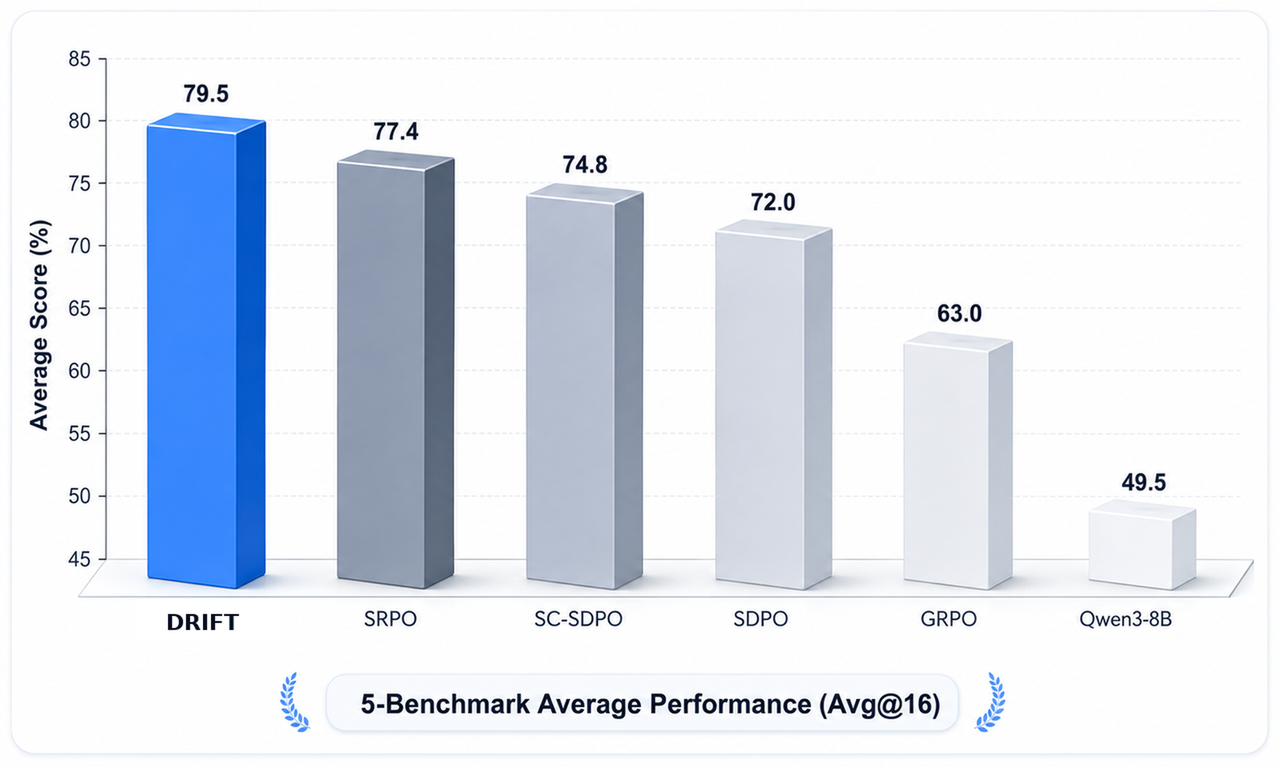
\includegraphics[width=\linewidth,height=4.5cm]{Figures/drift_performance.png}
        \caption{}
        \label{fig:fig1}
    \end{subfigure}
    \hspace{0.1cm}
    \begin{subfigure}[t]{0.42\textwidth}
        \centering
        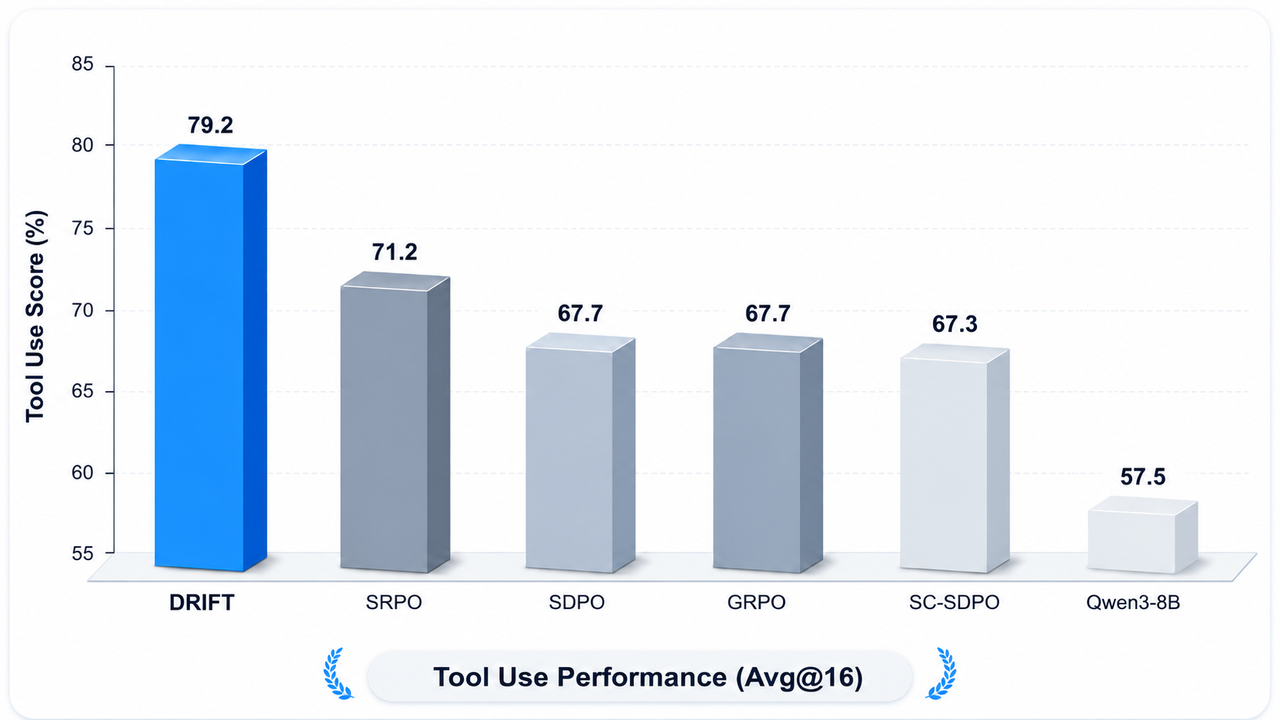
\includegraphics[width=\linewidth,height=4.5cm]{Figures/drift_convergence.png}
        \caption{}
        \label{fig:fig2}
    \end{subfigure}
    
    \caption{\textbf{DRIFT overview}}
    \label{fig:main}
\end{figure*}

\section{Introduction}

Recently, large language models (LLMs) have made remarkable progress on complex tasks such as mathematical reasoning, scientific problem solving, and tool use \cite{jaech2024learning,guo2025deepseekr1,deepseekai2026deepseekv4,comanici2025gemini25,olmo2025olmo3}. Beyond scaling pre-training, feedback-based reinforcement learning and self-distillation have emerged as important approaches for strengthening LLM reasoning\cite{shao2024deepseekmath,gu2023minillm,hubotter2026reinforcement,zhao2026opsd,jin2026entropyopd,fu2026revisitingopd,pan2026rlcsd,li2026rethinkingopd}. By learning from trajectories the model produces itself, these methods reduce the dependence on human expert demonstrations and offer a scalable route to self-evolution.

Despite their effectiveness, existing self-evolution paradigms share a key limitation: their training signals are rarely adapted to the model's evolving capability. Reinforcement learning methods such as GRPO~\citep{shao2024deepseekmath} encourage policy exploration through relative rewards, but the resulting updates can become noisy when successful samples are sparse or reward distributions are unstable. Self-distillation methods such as SDPO~\citep{hubotter2026reinforcement} reuse the model's correct solutions as supervision, yet they typically treat all such solutions uniformly, ignoring whether a problem is easy, near the model's capability boundary, or only occasionally solved. Recent sample-routing methods try to combine self-distillation with reinforcement learning~\citep{li2026srpo}, but most rely on immediate outcomes within the current batch and lack a persistent characterization of problem difficulty and learning progress \cite{zhang2025grpolead}. As a result, training signals are allocated suboptimally: already-mastered problems keep receiving redundant updates, hard problems fail to yield reliable supervision, and high-value boundary cases are under-explored~\cite{zhang2025grpolead,baroian2026prompt,hubotter2026reinforcement}. Compounding this, many methods neither retain nor reuse high-quality correct solutions across batches, preventing the formation of a durable memory for self-evolution~\citep{lin1992self,schaul2016prioritized,zhan2026exgrpo}.

To address these issues, we propose DRIFT, an online self-evolution policy optimization framework for LLMs. DRIFT adaptively coordinates self-distillation and reinforcement learning according to the model's estimated mastery of each problem, balancing error correction, exploration, and stable convergence. Using the model's own correct solutions as references, DRIFT routes each problem to a strategy matched to its difficulty: hard problems receive explicit distillation guidance, problems near the capability boundary drive reinforcement-learning exploration, and reliably solved problems are given fewer updates to avoid unnecessary policy perturbation. Crucially, a cross-batch memory retains high-quality correct solutions as distillation references, enabling hard problems rarely solved in the current batch to benefit from successful trajectories accumulated over time. DRIFT further refines reinforcement-learning updates through token-level modulation, concentrating policy improvement on the key positions in a reasoning trace that most directly determines reasoning quality. By integrating difficulty-aware signal allocation, token-level credit shaping, and cross-batch reuse of successful experience, DRIFT sustains a robust online self-evolution process without any external expert supervision.

We evaluate DRIFT by training Qwen3-8B~\citep{qwen3} on a diverse suite of tasks spanning biology, chemistry, materials, physics, and tool use. DRIFT clearly surpasses our reproduced SDPO and GRPO baselines and further improves over recent methods such as SRPO~\citep{li2026srpo}, with especially pronounced gains on the tool-use task.

Our contributions are as follows:
\begin{enumerate}
    \item \textbf{Dynamic Difficulty Routing.} Historical pass rates are used as a stable estimate of the model's mastery level, enabling dynamic decisions on when to distill from past successful trajectories, when to explore new strategies, and when to reduce redundant training.
    \item \textbf{Rhythm Gating Exploration.} A structure-preserving exploration mechanism is introduced to encourage policy variation near the success boundary, while preserving useful reasoning patterns through token-level Rhythm Gating.
    \item \textbf{Two-Stage Curriculum Learning.} A two-stage curriculum strategy is designed to align training behaviors with different phases of model learning. The first stage focuses on rapid capability growth and success buffer accumulation, allowing the model to reach a stable performance plateau efficiently. The second stage shifts toward balanced exploration, correction, and convergence, enabling continuous and stable performance improvement.
    \item \textbf{Experience Replay via Success Buffer.} DRIFT incorporates a historical success buffer to reuse high-quality trajectories. It further adopts a curriculum learning strategy to support smooth model evolution and uses Rhythm Gating to provide structured exploration rewards on boundary problems.
\end{enumerate}

\section{Preliminaries}

\subsection{GRPO and SDPO}

Group Relative Policy Optimization (GRPO) is a critic-free policy optimization method commonly used in post-training with verifiable rewards. Given a prompt $x$, the current policy samples a group of $G$ candidate rollouts. Each rollout receives a scalar reward, which is normalized within the group to compute its relative advantage $A_i^{\mathrm{GRPO}}$. The policy is then optimized using a PPO-style clipped surrogate objective, where $\rho_{i,t}(\theta)=\pi_\theta(y_{i,t}\mid x,y_{i,<t})/\pi_{\theta_{\mathrm{old}}}(y_{i,t}\mid x,y_{i,<t})$ denotes the token-level importance ratio:
\begin{equation}
\label{eq:grpo}
\mathcal{J}_{\mathrm{GRPO}}(\theta)=\mathbb{E}_{i,t}\left[\min\left(\rho_{i,t}(\theta)\,A_i^{\mathrm{GRPO}},\;\operatorname{clip}\left(\rho_{i,t}(\theta),1-\epsilon,1+\epsilon\right)A_i^{\mathrm{GRPO}}\right)\right].
\end{equation}
Since $A_i^{\mathrm{GRPO}}$ is computed at the sequence level, all tokens within the same rollout share the same advantage. Therefore, GRPO provides a trajectory-level reward alignment signal: high-reward responses are reinforced, while low-reward responses are suppressed. However, this also leads to coarse-grained credit assignment, as GRPO cannot directly identify which specific tokens are responsible for the final outcome.

Beyond the scalar reward, Self-Distillation Policy Optimization (SDPO) introduces dense token-level supervision from a self-teacher. Unlike methods that rely solely on the final outcome reward, SDPO leverages the model itself to construct a teacher distribution under additional feedback conditions, thereby providing the student with a finer-grained learning signal. The student policy can be written as $\pi_\theta(\cdot\mid x)$, whereas the self-teacher distribution is further conditioned on auxiliary feedback $f$, i.e., $\pi_\theta(\cdot\mid x,f)$. Here the feedback $f$ may arise from the rollout process---for instance, successful sibling responses within the same group of samples, verifier feedback, execution traces, or other auxiliary signals provided by the environment. Given a sampled trajectory $y_i$, SDPO compares the student and self-teacher distributions at the same prefix positions. We typically employ the Jensen--Shannon divergence (JSD), in which case the distillation loss can be written as:
\begin{equation}
\label{eq:sdpo}
\mathcal{L}_{\mathrm{SDPO}}(\theta)=\sum_t \mathrm{JSD}\left(\pi_\theta(\cdot\mid x,y_{i,<t})\,\big\Vert\, \operatorname{sg}\left[\pi_\theta(\cdot\mid x,f,y_{i,<t})\right]\right),
\end{equation}
\begin{equation}
\label{eq:jsd}
\mathrm{JSD}(P \,\|\, Q)= \frac{1}{2}\,\mathrm{KL}(P \,\|\, M)+ \frac{1}{2}\,\mathrm{KL}(Q \,\|\, M),\quad M = \frac{1}{2}(P+Q).
\end{equation}

Although GRPO and SDPO drive the self-improvement of large models along two paths---reinforcement learning and self-distillation, respectively---both struggle to adapt to the dynamic evolution of model capability. For GRPO, when intra-group rewards become homogeneous, the relative advantage weakens, leading to insufficient effective update signals. At the same time, all tokens within a single rollout share the same advantage in GRPO, so its credit assignment is too coarse-grained to localize the key reasoning steps that truly determine the outcome, causing a large portion of the updates to be spread over tokens unrelated to reasoning quality. By contrast, SDPO relies primarily on successful trajectories as the supervision signal, yet it usually treats all successful samples alike---neither distinguishing whether a sample comes from an easy problem, lies at the capability boundary, or is a hard problem solved by chance, nor characterizing problem-level learning progress. Such indiscriminate imitation may cause the model to keep producing redundant updates on easy problems it has already mastered, and to suppress exploration through a bias toward high-confidence behaviors; meanwhile, the boundary problems that carry genuine learning value are not sufficiently reinforced, and hard problems that lack successful trajectories cannot receive effective supervision. Ultimately, both GRPO and SDPO lack a mechanism that continually tracks the learning state at the problem level and dynamically allocates the optimization signal accordingly---which is precisely the core problem that DRIFT aims to address.

% ---- Section 3: Method ----
\section{Method}

\begin{figure}[t]
    \centering
    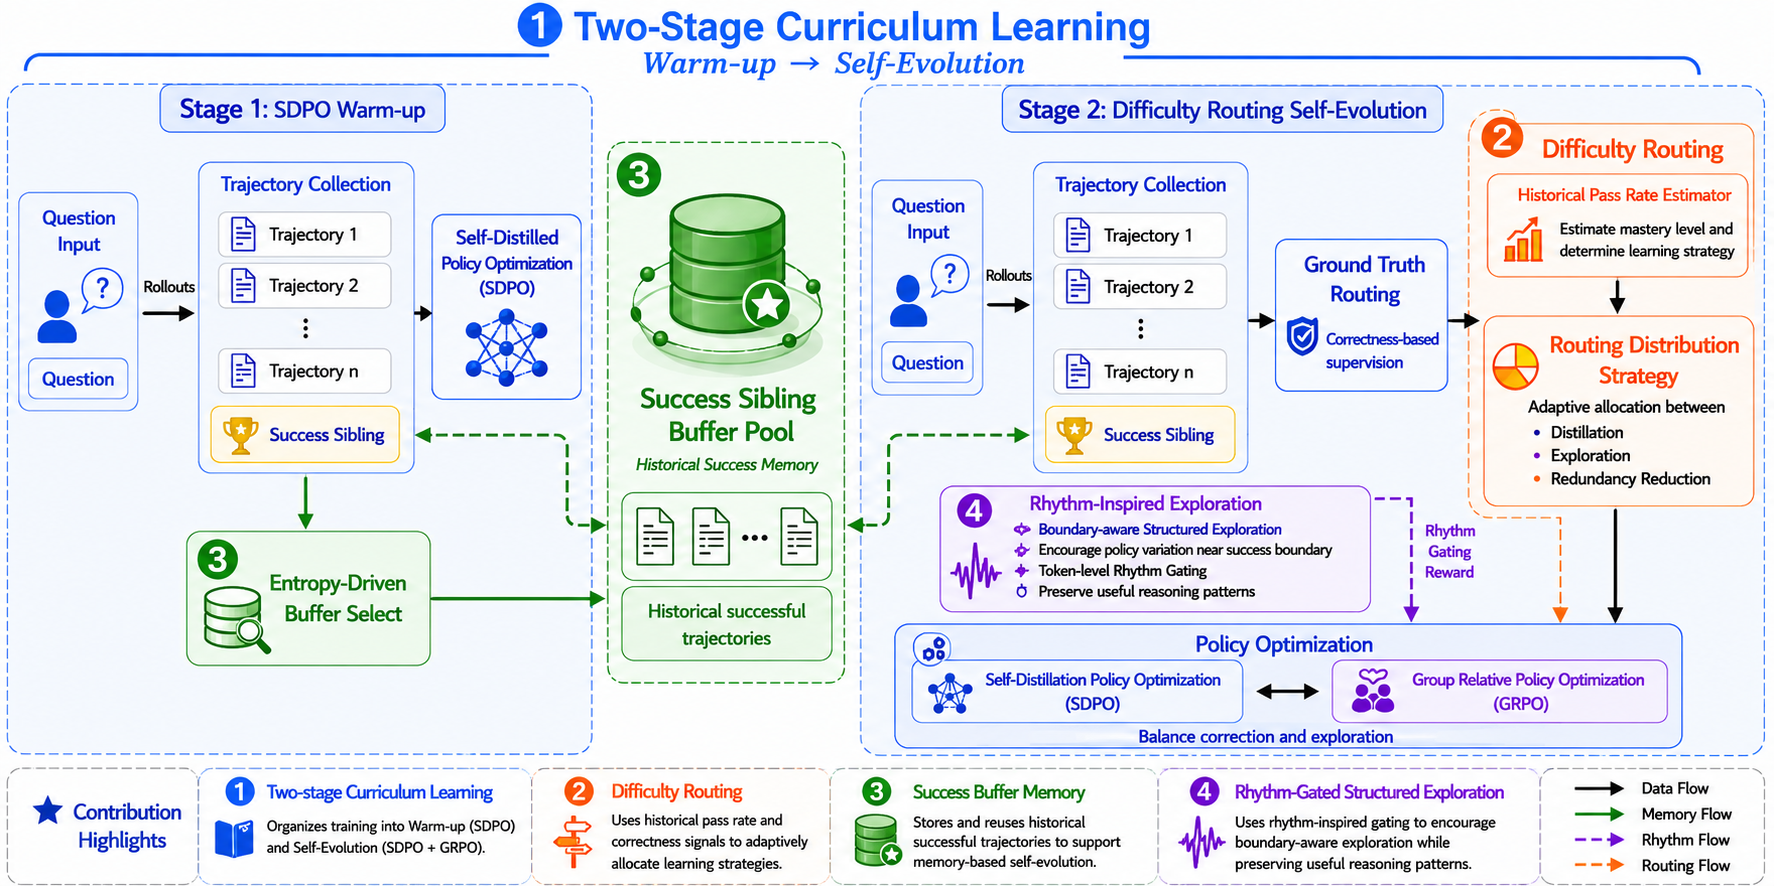
\includegraphics[width=0.95\linewidth]{Figures/drift_pipeline_new.png}
    \caption{Overall DRIFT training pipeline.}
    \label{fig:placeholder}
\end{figure}

DRIFT is built around these two levels and consists of three interlocking components: a \textbf{two-stage curriculum} that first uses self-distillation for a fast warm-up and to accumulate experience, and then switches to a stable optimization stage that combines self-distillation with reinforcement learning; a two-level signal refinement mechanism that dynamically allocates optimization signals at both levels: at the problem level, \textbf{difficulty routing} modulates the strength of reinforcement-learning updates according to the model's evolving mastery of each problem, while at the token level, \textbf{rhythm-gated structured exploration} concentrates credit on critical decision positions; and a privileged self-teacher that grows stronger throughout training, maintained jointly by the teacher-selection rule in the warm-up stage and a cross-stage \textbf{success buffer}, ensuring that dense token-level supervision remains available even when positive samples are scarce. We elaborate on each component below.

% ----------------------------------------------------------------
\subsection{Curriculum Teacher Construction}
\label{sec:curriculum}

DRIFT adopts a curriculum-learning organization that divides training into a warm-up stage and a mixed-optimization stage. The warm-up stage is dominated by SDPO, exploiting its higher sample efficiency relative to RL to rapidly improve model performance (pass@k) while simultaneously accumulating successful experience; the mixed stage then introduces the cooperation of SDPO and GRPO on top of this, continuing to improve capability in a more stable manner. The two stages share a single self-teacher played by the model itself, whose supervision is provided in the form of privileged information (a success sibling, denoted sib+).

\paragraph{Stage 1: Entropy-based teacher selection for the SDPO warm-up.}
In the warm-up stage we adopt an SDPO-dominated training framework. The difference from standard SDPO lies in the selection rule for the success sibling: standard SDPO fixes the choice to the first sample among all those satisfying $\text{reward}\ge\text{threshold}$, whereas we use a two-level ``reward-first, entropy-second'' strategy---we first select the sample with the largest reward, and then, among the samples with $\text{reward}\in[\,r_{\max}-\delta,\;r_{\max}\,]$, select the one with the largest entropy ($\delta$ being a tolerance). The reason we prefer 
a high-entropy successful trajectory as the teacher signal during warm-up is to maintain stronger exploration and diversity early in training, avoiding premature convergence to a single reasoning pattern. This stage has two goals: first, to leverage the high efficiency of SDPO for a fast performance warm-up; and second, to accumulate successful trajectories so as to build the success buffer, providing privileged supervision when positive samples are scarce in later stages.

\paragraph{Stage 2: Mixed optimization of SDPO and GRPO.}
In the mixed stage, we route samples into branches according to correctness: a sample with $\text{reward}<\theta_r$ is judged negative, and positive otherwise.
\begin{itemize}
  \item \textbf{Negative samples take the SDPO branch.} We select sib+ as the teacher to correct this erroneous trajectory. Unlike in warm-up, here we no longer prefer a high-entropy sib+; instead we prefer the one with the largest reward, and if several candidates share the same reward, we further prefer the one with the shortest response length---shorter responses usually have lower entropy, which helps the model converge. This stage emphasizes capability improvement over exploration, so the teacher-selection rule is adjusted accordingly. We do not apply pure GRPO to negative samples, because GRPO handles a negative sample by suppressing the generation probability of all of its tokens, which does not fully exploit the signal carried by the negative sample: the model is only told that ``the current trajectory is undesirable'' without learning in which direction it should be corrected, whereas sib+ provides a token-by-token correct path for comparison.
  \item \textbf{Positive samples take the rhythm-GRPO branch.} It should be emphasized that the sample advantage $A_i^{\text{GRPO}}$ is computed over all samples jointly, rather than only within the set of positive samples. The reason these samples take GRPO rather than SDPO is that using ``another correct trajectory'' to guide ``a trajectory that is already correct'' involves two inconsistent distributions, which may misguide the direction of policy adjustment and harm training stability; meanwhile, GRPO handles a positive sample by raising the generation probability of its current tokens, which more effectively preserves the model's existing capability.
\end{itemize}

Writing the two branches together, we obtain the overall objective of DRIFT in the mixed stage:
\begin{equation}
\label{eq:master}
\min_{\theta}\;\;\mathcal{L}(\theta):=
\mathbb{E}_{y_i\sim\pi_{\theta}(\cdot\mid x)}
\left[
\underbrace{
{\color{cIncorrect}\mathbf{1}_{y_i\in\mathrm{incorrect}}}\,
\mathcal{L}_{\mathrm{SDPO}}(y_i,f_i)
}_{\text{Self-Distillation}\;(\S\ref{sec:curriculum},\,\S\ref{sec:buffer})}
-
\underbrace{
{\color{cGamma}\gamma_i}\,
\mathbf{1}_{y_i\in\mathrm{correct}}\,
\mathcal{J}_{\mathrm{GRPO}}^{\mathrm{rhythm}}(y_i)
}_{\text{Difficulty-Routed RL}\;(\S\ref{sec:routing},\,\S\ref{sec:rhythm})}
\right],
\end{equation}
where the two branches expand respectively as
\begin{align}
\mathcal{L}_{\mathrm{SDPO}}(y_i,f_i)&:=\sum_{t=1}^{|y_i|}
\mathrm{JSD}\!\left(\pi_\theta(\cdot\mid x,y_{i,<t})\,\big\Vert\,
\sg\!\left[\pi_\theta(\cdot\mid x,f_i,y_{i,<t})\right]\right), \\[4pt]
\mathcal{J}_{\mathrm{GRPO}}^{\mathrm{rhythm}}(y_i)&:=\sum_{t=1}^{|y_i|}
{\color{cRhythm}M^{\mathrm{rhy}}_{t}}\cdot
\min\!\Big(\rho_{i,t}(\theta)\,A_i^{\text{GRPO}},\;
\mathrm{clip}\!\big(\rho_{i,t}(\theta),1-\epsilon,1+\epsilon\big)\,A_i^{\text{GRPO}}\Big).
\end{align}

This objective uses three colored terms to mark the division of labor among the following subsections: ${\color{cIncorrect}\mathbf{1}_{y_i\in\mathrm{incorrect}}}$ triggers the SDPO privileged-correction branch, whose teacher $f_i$ is provided jointly by the teacher-selection rule of this section and the success buffer of Section~\ref{sec:buffer}; ${\color{cGamma}\gamma_i}$ is the problem-level difficulty-routing weight, given by Section~\ref{sec:routing}; and ${\color{cRhythm}M^{\mathrm{rhy}}_{t}}$ is the token-level rhythm-gating weight, given by Section~\ref{sec:rhythm}. The following three subsections refine these three quantities in turn.

% ----------------------------------------------------------------
\subsection{Difficulty Routing}
\label{sec:routing}

This section refines the signal allocation at the problem level, i.e., ${\color{cGamma}\gamma_i}$ in the objective. Recent studies on RLVR/GRPO show that sample difficulty has a markedly non-monotonic effect on policy optimization: overly hard samples often fail to provide the most effective learning signal---positive trajectories are scarce among their rollouts, and even when a correct trajectory is occasionally sampled, it may be too far from the current model's capability or representation space to form a generalizable learning signal. We further observe that, in multiple-choice subject datasets, the model may guess the answer to a hard problem correctly while its chain-of-thought is in fact incorrect, which further miscalibrates the learning signal. Hence, easy and medium-difficulty samples are usually more suitable for GRPO~\citep{cheng2026sampledifficulty,baroian2026prompt}. On the other hand, overly easy problems tend to produce homogeneous rewards, leading to weak group-relative advantage signals; at the same time, such samples may mainly reinforce direct-answer or surface-level computation steps rather than deeper reasoning~\citep{chen2026unlearnability,cheng2026sampledifficulty}.

Accordingly, in the second stage of the curriculum we assign different weights to the positive samples taking the GRPO branch according to their difficulty: we reduce the GRPO update strength on overly easy and overly hard samples, and assign higher weight to medium-difficulty samples. Formally, this weight is exactly ${\color{cGamma}\gamma_i}$ in the objective, taking different values according to problem difficulty.

\paragraph{Computation and smoothing of the pass rate.}
We use a problem's pass rate as the basis for difficulty partitioning. The most direct way is to use the success rate of the current sample as the pass rate,
\begin{equation}
r_{\mathrm{now}} = \frac{n_{\mathrm{correct}}}{n},
\end{equation}
where $n$ is the number of rollouts for a single sample. However, since $n$ is usually small (8 or 16), the $r_{\mathrm{now}}$ estimated at different epochs may fluctuate too much even when the model is fixed, causing unstable difficulty partitioning. We therefore smooth it with an exponential moving average (EMA) of the historical pass rate:
\begin{equation}
r = \alpha\, r_{\mathrm{past}} + (1-\alpha)\, r_{\mathrm{now}}.
\end{equation}

\paragraph{Difficulty binning and weight values.}
Using the smoothed pass rate $r$, we partition problems into easy, medium, and hard, and take a different ${\color{cGamma}\gamma_i}$ for each:
\begin{itemize}
  \item \textbf{Easy}: $r > r_{\mathrm{easy}}$, take $\gamma_i = \gamma_{\mathrm{easy}}$;
  \item \textbf{Medium}: $r_{\mathrm{hard}} < r < r_{\mathrm{easy}}$, take $\gamma_i = 1$;
  \item \textbf{Hard}: $r < r_{\mathrm{hard}}$, take $\gamma_i = \gamma_{\mathrm{hard}}$.
\end{itemize}
In our numerical experiments we generally set $\gamma_{\mathrm{hard}}=0,\ \gamma_{\mathrm{easy}}=0.5,\ r_{\mathrm{easy}}=0.8,\ r_{\mathrm{hard}}=0.2$. This routing directly addresses the problem-level gap pointed out in the Introduction: for easy problems (homogeneous rewards, vanishing advantage) it suppresses redundant updates and surface-level reinforcement; for hard problems (scarce positives, accidental correctness) it avoids being misguided by miscalibrated signals; and it concentrates the effective reinforcement-learning budget on the medium-difficulty region with the highest learning value.

% ----------------------------------------------------------------
\subsection{Rhythm-Gated Structured Exploration}
\label{sec:rhythm}

This section refines the credit assignment at the token level, i.e., ${\color{cRhythm}M^{\mathrm{rhy}}_{t}}$ in the objective. Standard GRPO uses only the sequence-level advantage and cannot distinguish differences in token importance within the reasoning structure: a large number of semantically irrelevant tokens (e.g., formatting symbols, high-frequency connectives) share the same exploration signal as critical decision tokens, which both introduces gradient noise and skews credit assignment away from the reasoning steps that truly determine correctness. To improve the effectiveness of the exploration signal within the medium-difficulty region, we introduce a \textbf{rhythm-gated rebellious bonus} on the GRPO branch determined by difficulty routing: we construct a token-level estimate of structural salience from the difference in temporal entropy dynamics between teacher and student, and then use this salience to gate the student's local exceedance over the teacher. This mechanism does not uniformly amplify the policy gradient of all correct samples; rather, it applies a bounded amplification to a local token update only when two conditions hold simultaneously---first, the sample lies in the medium-difficulty region ``worth continuing to explore''; and second, a token position exhibits both a local exceedance of the student over the teacher and a high structural salience. This improves the effectiveness and interpretability of exploratory updates while controlling the magnitude of optimization perturbations.

Overall, the final token weight is determined by the product of two factors: one characterizing the \textbf{local exceedance strength} of the student relative to the teacher (the rebellious bonus), and the other characterizing the \textbf{structural salience} of the position (the anchor rhythm gate). We construct each in turn.

\paragraph{Local exceedance: teacher-relative rebellious bonus.}
Let $\ell_t^S$ and $\ell_t^T$ denote the log-probabilities assigned by the student and the teacher, respectively, to the actually sampled token at the $t$-th response token. Define the local exceedance of the student relative to the teacher as
\begin{equation}
\Delta_t=\ell_t^S-\ell_t^T-\mu,
\qquad
\Delta_t^{+}=\max(\Delta_t,0),
\end{equation}
where $\mu\ge 0$ is a margin used to filter out overly small random fluctuations. On top of this we construct a bounded rebellious bonus
\begin{equation}
B_t=\min\!\big(\exp(\tau\,\Delta_t^{+}),\, B_{\max}\big),
\qquad
b_t^{\mathrm{reb}}=B_t-1,
\end{equation}
where $\tau>0$ is a temperature coefficient and $B_{\max}$ gives an upper bound. This quantity only answers ``whether the student significantly surpasses the teacher at this token,'' and does not distinguish whether the token is truly important; if applied indiscriminately to all positions with $\Delta_t>0$, the model might allocate too much gradient budget to semantically neutral tokens such as formatting symbols and connectives, thereby amplifying ineffective exploration.

\paragraph{Structural salience: anchor rhythm gate.}
To this end we introduce an anchor rhythm gate that acts only on the rebellious bonus. It does not directly weight the SDPO distillation loss, but serves only as a structural filter for the rebellious bonus on the GRPO branch; this temporal-anchor signal combines past and future information simultaneously, so as to more accurately capture the rhythmic key points of exploration. Let $H_t^S$ and $H_t^T$ be the token entropies of the student and the teacher at position $t$. For a local window of length $W$, define the entropy collapse of model $*\in\{S,T\}$ near this position as
\begin{equation}
\mathrm{Drop}_*(t)=\max\!\big(\bar H^{*}_{\mathrm{past}}(t)-\bar H^{*}_{\mathrm{future}}(t),\,0\big).
\end{equation}
If the teacher exhibits a more pronounced local entropy collapse than the student near position $t$, while the student is still more uncertain than the teacher at that position, then the position is more likely to be an ``anchor'' in the reasoning structure. Accordingly, we define the anchor score
\begin{equation}
D_t^{\mathrm{anc}}
=
\max\!\big(\mathrm{Drop}_T(t)-\mathrm{Drop}_S(t),\,0\big)
\cdot
\max\!\big(H_t^S-H_t^T,\,0\big).
\end{equation}
We then apply z-score normalization to $D_t^{\mathrm{anc}}$ within each sequence, and map it to $[0,1]$ via a soft gate:
\begin{equation}
z_t^{\mathrm{anc}}=\zscore_{\mathrm{seq}}(D_t^{\mathrm{anc}}),
\qquad
g_t^{\mathrm{anc}}
=
2\max\!\left(\sigma(\alpha_{\mathrm{anc}}\, z_t^{\mathrm{anc}})-\tfrac12,\,0\right).
\end{equation}
Define the anchor rhythm multiplier $m_t = 1 + \lambda_{\mathrm{struct}}\, g_t^{\mathrm{anc}}$, and apply within-sequence mean normalization and clipping
\begin{equation}
\tilde m_t=\frac{m_t}{\tfrac{1}{|Y|}\sum_{j\in Y}m_j},
\qquad
m_t^{\mathrm{clip}}=\mathrm{clip}(\tilde m_t,\, m_{\min},\, m_{\max}),
\end{equation}
and then linearly map it to the final gate
\begin{equation}
g_t^{\mathrm{rhythm}}
=
\mathrm{clip}\!\left(
\frac{m_t^{\mathrm{clip}}-1}{m_{\max}-1},\,0,\,1
\right).
\end{equation}
In this way, only positions whose structural salience is above the within-sequence average receive a positive rhythm gate, while tokens below the mean or in the neutral region are filtered out directly.

\paragraph{Composite weight and double screening.}
Combining the two factors, the token weight actually used on the GRPO branch is
\begin{equation}
\label{eq:rhy-weight}
{\color{cRhythm}M^{\mathrm{rhy}}_{i,t}}
=
1+\beta_i \, g_{i,t}^{\mathrm{rhythm}} \, b_{i,t}^{\mathrm{reb}},
\end{equation}
where $\beta_i$ is a sample-level medium-difficulty indicator: $\beta_i=1$ if and only if sample $i$ is routed as medium by Section~\ref{sec:routing}, and $\beta_i=0$ for easy and hard. This expression clearly reflects the division of labor among the three types of signals: $\beta_i$ decides at the sample level whether the sample belongs to the medium-difficulty region worth exploring, $b_{i,t}^{\mathrm{reb}}$ measures whether the student achieves a local exceedance over the teacher at this token, and $g_{i,t}^{\mathrm{rhythm}}$ judges whether this exceedance occurs at a structurally more critical position. In other words, this mechanism performs a kind of ``double screening'' at the token level: it first detects whether a teacher-relative improvement exists, and then detects whether that improvement falls on a high-value structural anchor. Rhythm does not change the direction of the distillation objective; it serves only as a structural gate for the rebellious bonus, keeping the exploration enhancement local, bounded, and low-risk.

This design is supported by three considerations. First, \textbf{exploration should be teacher-relative} rather than unconditionally amplifying all correct tokens: in the medium-difficulty region, the model already has a certain success rate but has not yet converged stably, and the most valuable signal here is often not ``what the teacher already knows'' but ``at which local positions the student begins to significantly surpass the teacher.'' Hence the rebellious bonus is defined by the relative difference $\ell_t^S-\ell_t^T$, granting extra gain only when the student's support for the actually sampled token is clearly stronger than the teacher's, thereby focusing exploration on positions where the student's new capabilities are emerging, rather than treating the teacher as an insurmountable upper bound. Second, \textbf{a local exceedance does not automatically imply a high-value exceedance}: language models may occasionally achieve a higher log-prob on low-semantic-load tokens such as formatting symbols, connectives, and repeated phrases, and if all positions with $\Delta_t>0$ are treated equally, the training signal will be diluted by a large number of ``surface-level exceedances,'' skewing credit assignment away from the key positions that determine correctness; the role of the rhythm gate is not to introduce a second independent reward, but to answer a finer question---whether the exceedance occurs at a structurally worthwhile position. Third, the \textbf{intuition of the temporal anchor} is that, at the key turning points of a reasoning chain, the teacher often completes the local collapse of uncertainty faster than the student, and if the student is still more uncertain at this moment, the position is very likely a structural anchor that the student has not yet stably mastered; retaining the rebellious bonus only at such positions amounts to reallocating the exploration budget from ``all seemingly better tokens'' to ``the tokens more likely to determine future reasoning success or failure.'' Taken together, this mechanism is a two-stage but single-path token-level credit-assignment process: the first stage detects, via the rebellious term, whether a teacher-relative improvement occurs, and the second stage detects, via the anchor rhythm gate, whether that improvement falls at a position of high structural value; a token receives extra amplification only when both hold---preserving the progressiveness of teacher-relative exploration while constraining its variance and noise propagation through the structural gate, forming a local and bounded exploration enhancement suitable for the medium-difficulty boundary region.

% ----------------------------------------------------------------
\subsection{Success Buffer}
\label{sec:buffer}

Finally, we explain how to keep the privileged self-teacher always present and increasingly strong, i.e., how to still provide $f_i$ for the SDPO branch when positive samples are scarce. Inspired by RLEP~\citep{zhang2025rlep}, we introduce a success buffer mechanism into OPD. RLEP shows that, in reinforcement learning for large-model reasoning, trajectories that have been verified as correct can be reused via experience replay, so that the policy need not explore from scratch at every update but can continually reinforce existing effective reasoning paths. Building on this idea, we store rollouts that obtain a positive verification signal into a buffer during sampling, and replay the successful samples within it as sib+ in subsequent OPD updates, injecting them into training in the form of privileged information. Unlike the offline, static replay buffer in RL, our buffer is dynamically replaced: since the teacher's capability keeps growing and rewards keep rising throughout training, the sib+ corresponding to the same problem in the buffer is replaced by higher-quality trajectories as training proceeds; this amounts to introducing, in the form of privileged information, an implicit reward signal that strengthens with training, rather than simply replaying fixed historical experience.

The specific design is as follows. In the first $k$ epochs of training, we encourage the model to explore freely, only accumulating the success buffer without using it; from the $(k{+}1)$-th epoch onward, the buffer's data are used as sib+ only when no sib+ can be found within a group of rollouts; each data point stores at most $b$ sib+ simultaneously (we take $b=3$ in experiments), and one of them is randomly chosen at use time; when the sib+ of a data point is full, replacement is done by reward, with high-reward sib+ replacing low-reward ones.

Formally, for each training sample $x$ we maintain a success buffer
\begin{equation}
\mathcal{B}(x)=\{(y_j^+, r_j)\}_{j=1}^{m_x},
\qquad m_x \le b,
\end{equation}
where $\{y_j^+\}$ are historical successful rollouts and $\{r_j\}$ are their corresponding rewards. In the first $k$ epochs, the buffer is only updated, not used:
\begin{equation}
i \le k:\qquad
\mathcal{B}(x) \leftarrow \mathrm{Update}\big(\mathcal{B}(x),\, y^+,\, r(y^+)\big).
\end{equation}
From the $(k{+}1)$-th epoch onward, given a set of rollouts $\mathcal{Y}(x)=\{y_1,\dots,y_n\}$ obtained by current sampling, if the set contains no successful rollout, i.e.,
\begin{equation}
\{\,y_i \in \mathcal{Y}(x): r(y_i)>0\,\}=\varnothing,
\end{equation}
then a historical successful sibling is randomly sampled from the buffer as the sib+ for the current sample:
\begin{equation}
\tilde{y}^+ \sim \mathrm{Uniform}\big(\mathcal{B}(x)\big).
\end{equation}
The buffer is updated by a reward-based replacement mechanism. When the buffer is not full, a new successful rollout is added directly:
\begin{equation}
|\mathcal{B}(x)|<b:\qquad
\mathcal{B}(x) \leftarrow \mathcal{B}(x)\cup \{(y^+, r(y^+))\}.
\end{equation}
When the buffer is full, let $j^\star = \arg\min_j r_j$ denote the index of the entry with the lowest reward; then
\begin{equation}
\mathcal{B}(x) \leftarrow
\begin{cases}
\big(\mathcal{B}(x)\setminus \{(y_{j^\star}^+, r_{j^\star})\}\big)\cup \{(y^+, r(y^+))\},
& \text{if } r(y^+) > r_{j^\star}, \\[4pt]
\mathcal{B}(x),
& \text{otherwise}.
\end{cases}
\end{equation}

This mechanism increases the utilization of high-quality generated samples, reduces the sample waste caused by discarding successful rollouts at once, and provides a more stable positive training signal for the student policy. Unlike standard on-policy training, where a rollout is discarded after a single update, our framework retains successful reasoning trajectories and reuses them as auxiliary signals for policy distillation and optimization. It is worth noting that the memory overhead of maintaining the success buffer is small: since the buffer is essentially a plain-text dictionary, its footprint grows as (number of problems) $\times$ (successful entries per problem) $\times$ (per-response length), amounting to at most about $0.2$--$0.3$\,GB under our default configuration and typically staying within a few hundred MB in practice---negligible compared with the model weights and optimizer states, and thus it does not adversely affect training.

\section{Experiments}

\subsection{Experimental Setup}

\paragraph{Models and training.}
We conduct experiments on three instruction-tuned models, including Qwen3-8B~\citep{qwen3}, Qwen3-4B, and OLMo3-7B~\citep{olmo2025olmo3}, covering both different scales within the same model family and models from different families. Qwen3-8B serves as our primary model; unless otherwise noted, all ablation studies and training-dynamics analyses beyond the main performance comparison are conducted on Qwen3-8B. All experiments are trained for more than400 steps on 8 NVIDIA H200 GPUs. 
Unlike prior work that reports results in terms of wall-clock time~\citep{hubotter2026reinforcement,li2026srpo}, we follow SC-SDPO~\citep{liu2026scsdpo} and report results in terms of training steps, since optimization steps are independent of hardware configuration and enable reproducible comparison across different compute environments.

\paragraph{Datasets.}
Following the evaluation setting of SDPO, we conduct experiments on five benchmarks: Chemistry, Physics, Biology, Materials, and Tool Use. The first four benchmarks are drawn from the reasoning subsets of SciKnowEval~\citep{feng2024sciknoweval}, covering undergraduate-level scientific reasoning across multiple domains. The Tool Use benchmark assesses the model's ability to convert a user query and a given tool specification into the correct tool invocation, following ToolAlpaca~\citep{tang2023toolalpaca}. Following SDPO, we split each benchmark into training and test sets to measure in-domain generalization.

\paragraph{Baselines.}
We compare DRIFT with six baselines: GRPO~\citep{shao2024deepseekmath}, SDPO~\citep{hubotter2026reinforcement}, SRPO~\citep{li2026srpo}, DistIL~\citep{agrawal2026distil}, SC-SDPO~\citep{liu2026scsdpo}, and PGPO~\citep{wang2026pgpo}. We reproduce GRPO and SDPO using the implementation framework provided by SDPO~\citep{hubotter2026reinforcement}, with the default hyperparameter settings kept unchanged. For SRPO, DistIL, SC-SDPO, and PGPO, we use the results reported in their corresponding papers~\citep{li2026srpo, agrawal2026distil, liu2026scsdpo, wang2026pgpo}. When comparing with reported numbers, we follow the same benchmark and evaluation protocol whenever applicable.

% Keep enough room for the wrapped figure and its caption. If necessary,
% move the block to the next page without reserving excessive blank space.
\Needspace{0.16\textheight}
\subsection{Main Results}

% Right-side figure with the main-results text wrapped around it.
\begin{wrapfigure}[10]{r}{0.38\textwidth}
    \vspace{-1.5\baselineskip}
    \centering
    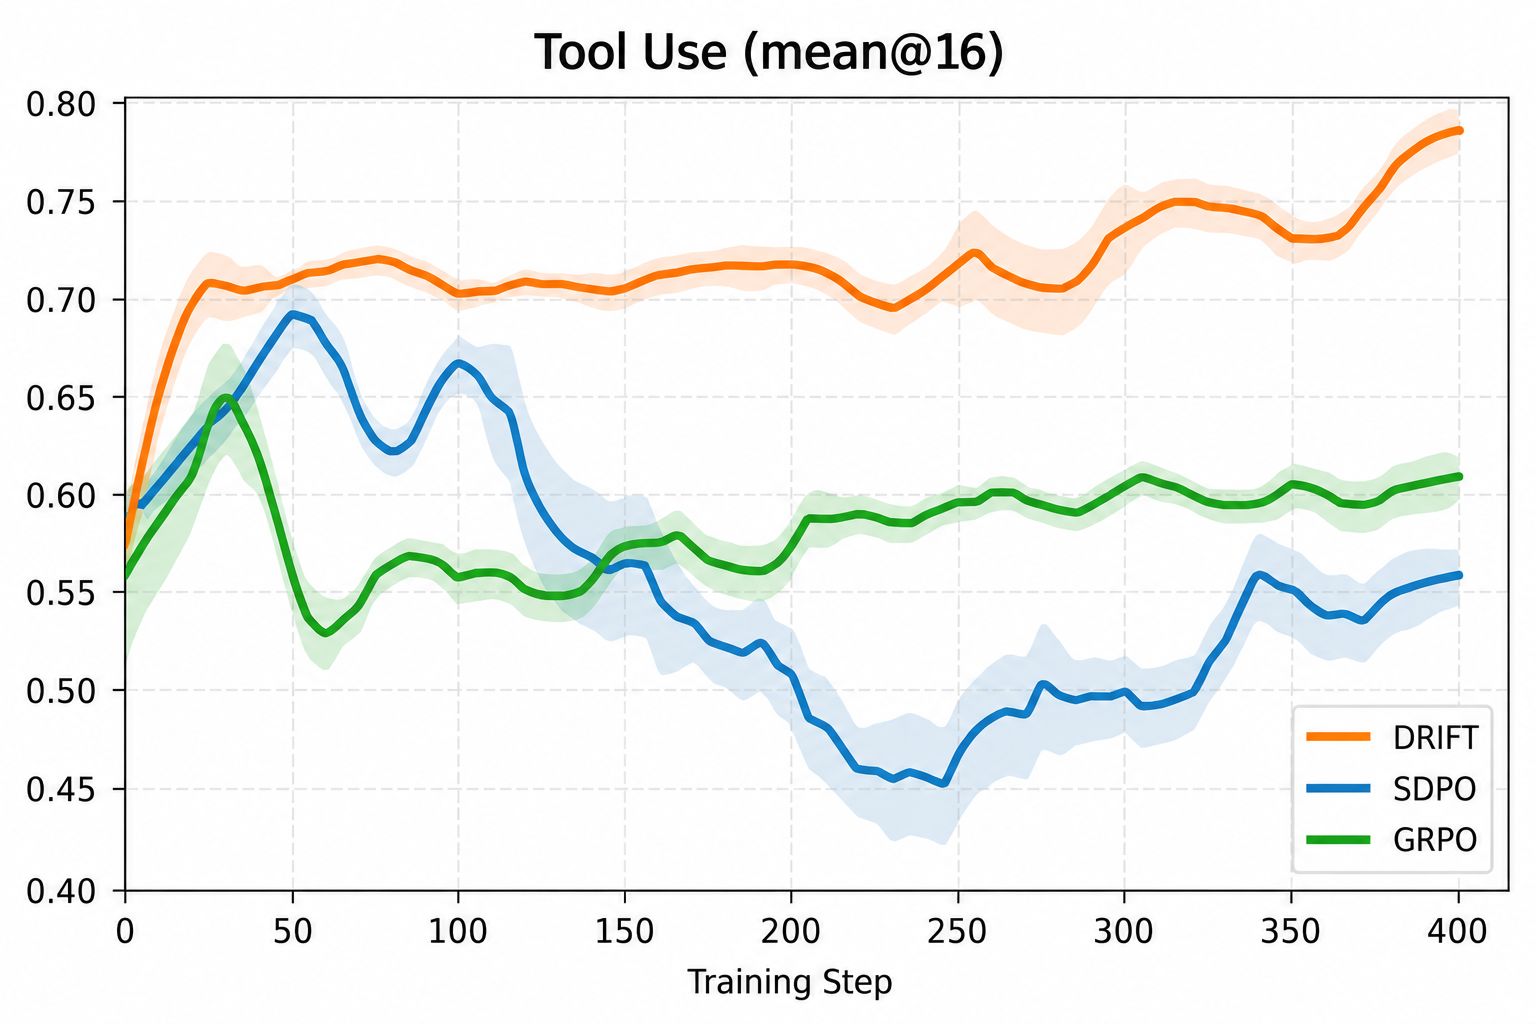
\includegraphics[width=\linewidth]{Figures/drift_tooluse_plot.png}
    \captionsetup{font=scriptsize,skip=2pt}
    \caption{\textbf{Tool-use performance}}
    \label{fig:fig3}
    \vspace{-1.0\baselineskip}
\end{wrapfigure}

\paragraph{Main results.}
Our main results are reported as the mean@16 accuracy of Qwen3-8B across four scientific reasoning tasks (biology, chemistry, materials, physics) and tool use. DRIFT attains the highest average accuracy of 79.5\%, outperforming the previously strongest baseline SRPO (77.4\%) by 2.1 points, SC-SDPO (74.8\%) by 4.7 points, and the GRPO/SDPO-series baselines by 7.5--9.5 points, while improving over the Qwen3-8B starting point (49.5\%) by 30.0 points. Beyond the overall average, DRIFT is the only method that ranks in the top two on every task: it is best on biology (74.4\%) and tool use (79.2\%), and second-best on chemistry (82.0\%), materials (81.4\%), and physics (80.5\%), with a gap of no more than 1.1 points from the per-task optimum. This balance arises from the targeted treatment of the learning signal afforded by difficulty routing: on hard tasks, GRPO suffers from advantage collapse because the entire group receives the same reward and can only suppress incorrect trajectories indiscriminately, whereas DRIFT routes such cases to the SDPO branch and leverages sib+ to provide token-level correction (on the hardest task, biology, our GRPO reproduction reaches only 47.4\%, while DRIFT attains 74.4\%); on easier samples, it applies difficulty weighting to curb superficial reinforcement. By contrast, other methods tend to be uneven across tasks (e.g., SC-SDPO leads on physics but drops to 65.4\%/67.3\% on biology/tool use). The improvement is most pronounced on tool use, where DRIFT leads the second-best SRPO by 8.0 points.

DRIFT's effectiveness stems from its balance between exploration and structured knowledge learning. The self-distillation branch converts successful in-group siblings into structured supervision, enabling the model to reliably absorb reusable knowledge such as tool protocols, domain facts, and standardized answer formats. Meanwhile, the rhythm-gated rebellious mechanism preserves controlled exploration in the policy-gradient branch, preventing premature convergence to specific successful trajectories. Together, these two components allow DRIFT to improve performance on both tool-use and STEM datasets. The larger gains on tool-use tasks arise because correctness there is clearly defined by tool schemas, \texttt{Action}/\texttt{Action Input} formats, and argument constraints; successful demonstrations are highly standardized and easily reusable across samples, yielding cleaner distillation signals and more stable correction. In contrast, structured knowledge in STEM tasks is more tightly coupled with problem-specific content, making it less reusable and leading to comparatively more moderate gains.

\begin{table}[tbp]
\centering
\small
\caption{Comparison of different post-training methods based on Qwen3-8B, reported as mean@16 accuracy (\%). Results marked with $\ast$ are cited from prior work. \textbf{Bold} and \underline{underlined} values indicate the best and second-best results, respectively. {\color{impgreen}Green subscripts} denote absolute gains over the reproduced SDPO baseline.}
\label{tab:main_qwen3_8b}
\begin{tabular}{lcccccc}
\toprule
Method & Biology & Chemistry & Material & Physics & Tool Use & Average \\
\midrule
\textbf{Qwen3-8B} & 30.8 & 41.2 & 58.9 & 59.2 & 57.5 & 49.5 \\
+ SDPO$^{\ast}$ & 56.8 & 80.9 & 78.4 & 75.6 & 68.5 & 72.0 \\
+ SDPO & 64.8 & 78.9 & 76.1 & 72.7 & 67.7 & 72.0 \\
+ GRPO$^{\ast}$ & 59.9 & 74.5 & 77.1 & 72.7 & 65.7 & 70.0 \\
+ GRPO & 47.4 & 65.6 & 73.5 & 60.6 & 67.7 & 63.0 \\
+ SRPO$^{\ast}$ & \underline{72.8} & \textbf{83.0} & \textbf{81.5} & 78.4 & \underline{71.2} & \underline{77.4} \\
+ DistIL$^{\ast}$ & 66.6 & 80.8 & 76.2 & \underline{80.8} & -- & -- \\
+ SC-SDPO$^{\ast}$ & 65.4 & 80.6 & 79.3 & \textbf{81.6} & 67.3 & 74.8 \\
+ PGPO$^{\ast}$ & 61.3 & 77.6 & 78.7 & 77.6 & -- & -- \\
\midrule
\textbf{+ DRIFT (Ours)} & \textbf{74.4}\imp{9.6} & \underline{82.0}\imp{3.1} & \underline{81.4}\imp{5.3} & 80.5\imp{7.8} & \textbf{79.2}\imp{11.5} & \textbf{79.5}\imp{7.5} \\
\bottomrule
\end{tabular}
\end{table}

\paragraph{Generalization across model families and scales.}
On Qwen3-4B and Olmo3-7B, DRIFT again attains the highest average accuracy (74.6\% and 72.8\%), and its advantage on tool use remains the largest (leading the second-best by 7.0 and 7.3 points, respectively). We highlight two observations. First, the gain amplifies as the starting point weakens: on Olmo3-7B (base 30.5\%), DRIFT improves by 42.3 points and leads online GRPO by 12 points, because when positive samples are scarce, the privileged replay from the success buffer fills exactly the void left by GRPO's advantage collapse. Second, the lead over the strongest baseline SRPO widens with scale (+0.4 at 4B, +2.1 at 8B), consistent with the observation that self-teaching ability emerges with increasing model scale.

\begin{table}[tbp]
\centering
\small
\caption{Comparison of different post-training methods on Qwen3-4B and Olmo3-7B, reported as mean@16 accuracy (\%). We use the same notation as in Table~\ref{tab:main_qwen3_8b}.}
\label{tab:main_qwen4b_olmo7b}
\begin{tabular}{lcccccc}
\toprule
Method & Biology & Chemistry & Material & Physics & Tool Use & Average \\
\midrule
\textbf{Qwen3-4B} & 30.8 & 43.6 & 61.2 & 59.8 & 57.9 & 50.7 \\
+ SDPO$^{\ast}$ & 54.0 & 77.3 & 74.3 & 66.7 & 61.1 & 66.7 \\
+ GRPO$^{\ast}$ & 55.5 & 78.3 & 80.1 & 71.9 & 62.9 & 69.7 \\
+ SRPO$^{\ast}$ & \textbf{65.8} & \textbf{82.7} & \underline{81.3} & \textbf{74.0} & \underline{67.0} & \underline{74.2} \\
\textbf{+ DRIFT (Ours)} & \underline{64.3}\imp{10.3} & \underline{79.6}\imp{2.3} & \textbf{82.8}\imp{8.5} & \underline{72.2}\imp{5.5} & \textbf{74.0}\imp{12.9} & \textbf{74.6}\imp{7.9} \\
\midrule
\textbf{Olmo3-7B} & 16.2 & 22.8 & 36.7 & 37.7 & 39.3 & 30.5 \\
+ SDPO$^{\ast}$ & 52.8 & 80.0 & \underline{79.1} & 66.1 & 62.1 & 68.0 \\
+ GRPO$^{\ast}$ & 49.8 & 57.5 & 73.5 & 62.7 & 60.6 & 60.8 \\
+ SC-SDPO$^{\ast}$ & \underline{55.9} & \underline{81.5} & \underline{79.1} & 71.1 & \underline{62.9} & \underline{70.1} \\
+ DistIL$^{\ast}$ & 55.3 & 81.0 & 76.9 & \textbf{74.5} & -- & -- \\
\textbf{+ DRIFT (Ours)} & \textbf{61.3}\imp{8.5} & \textbf{82.0}\imp{2.0} & \textbf{79.2}\imp{0.1} & \underline{71.3}\imp{5.2} & \textbf{70.2}\imp{8.1} & \textbf{72.8}\imp{4.8} \\
\bottomrule
\end{tabular}
\end{table}

\subsection{Training Dynamics}

\begin{figure}[tbp]
    \centering
    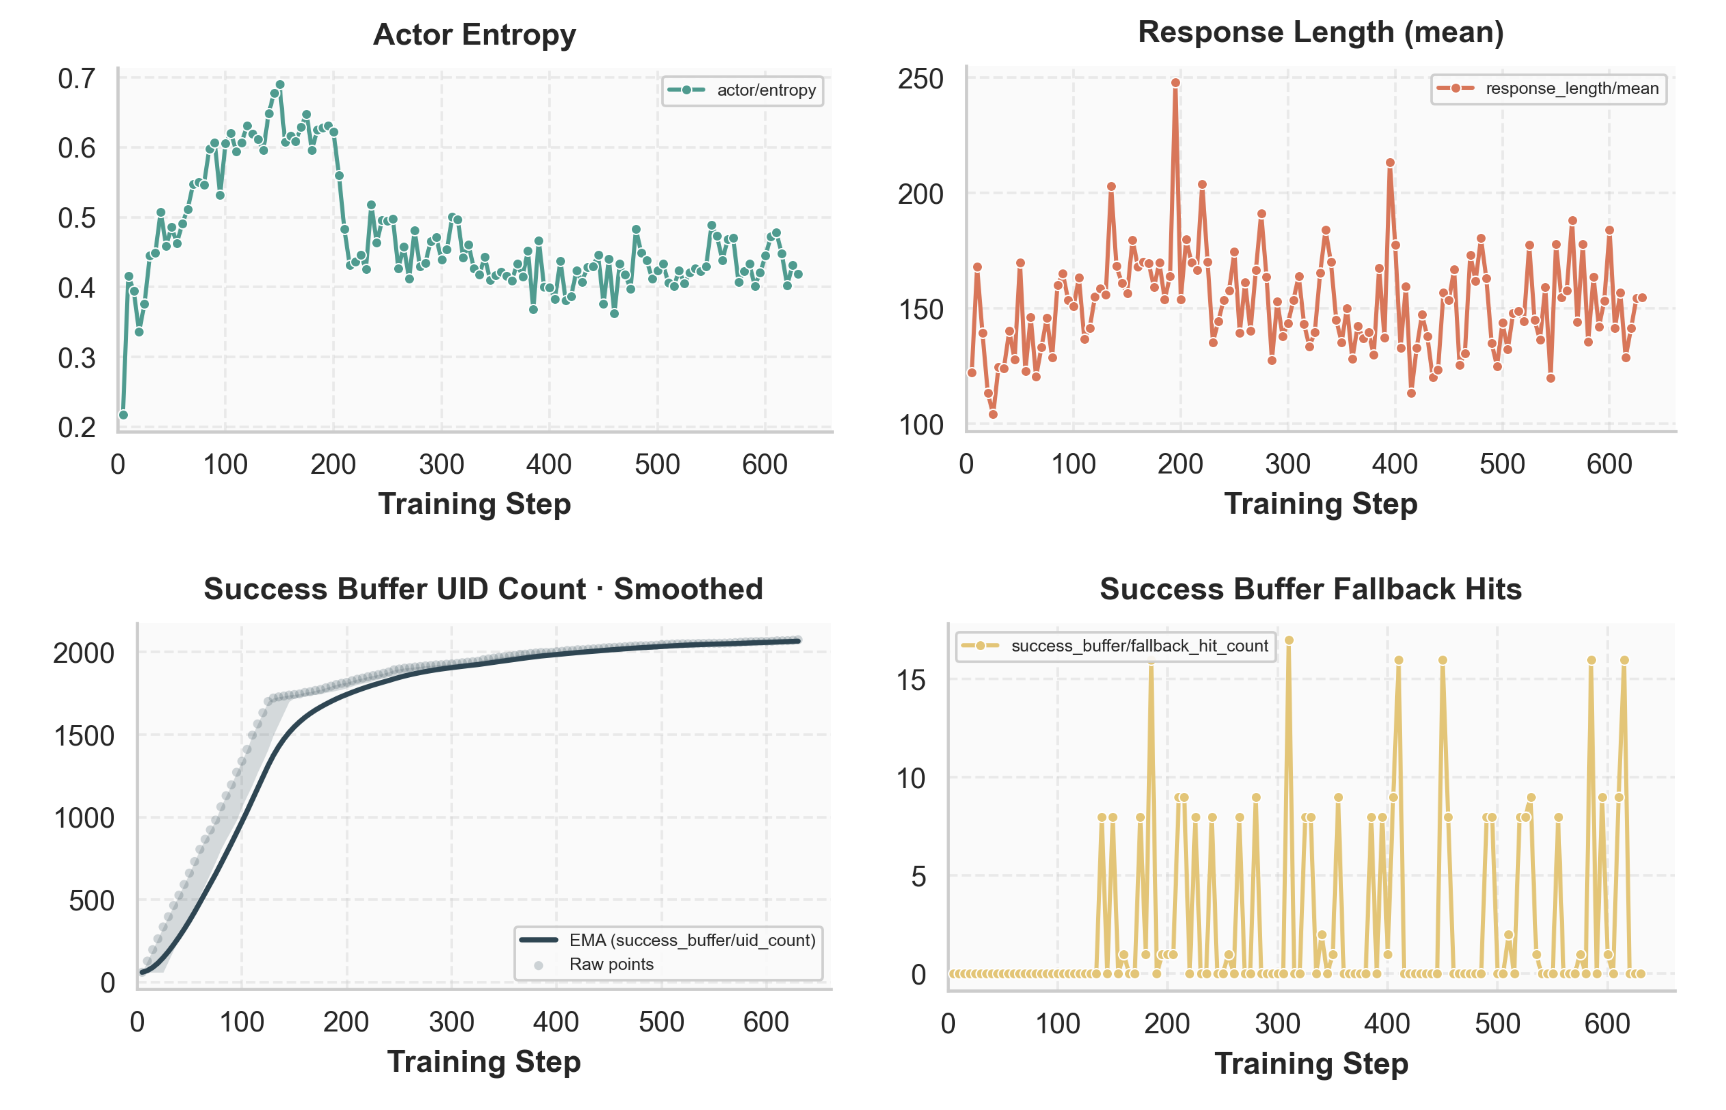
\includegraphics[width=0.86\textwidth]{Figures/drift_training_dynamics.png}
    \caption{\textbf{Training dynamics of DRIFT (Qwen3-8B in tooluse)}}
    \label{fig:training_dynamics}
\end{figure}

\paragraph{Training dynamics.}
Figures~\ref{fig:training_dynamics} and~\ref{fig:routing_dynamics} summarize the evolution of DRIFT during training. Actor entropy rises during early exploration and stabilizes after approximately 200 steps, while response length remains bounded. The success buffer grows rapidly before approaching saturation, with intermittent fallback hits indicating selective reuse of historical successes. At the same time, the easy-problem fraction gradually increases, the medium group remains dominant, and the hard fraction declines before stabilizing. Together, these trends show that DRIFT progressively shifts from broad exploration toward stable refinement while continuously adapting its routing decisions to the model's evolving capability.

\begin{figure}[tbp]
    \centering
    % 将 0.98 改为 1.1 或更大，图片会向两边页边距延伸
    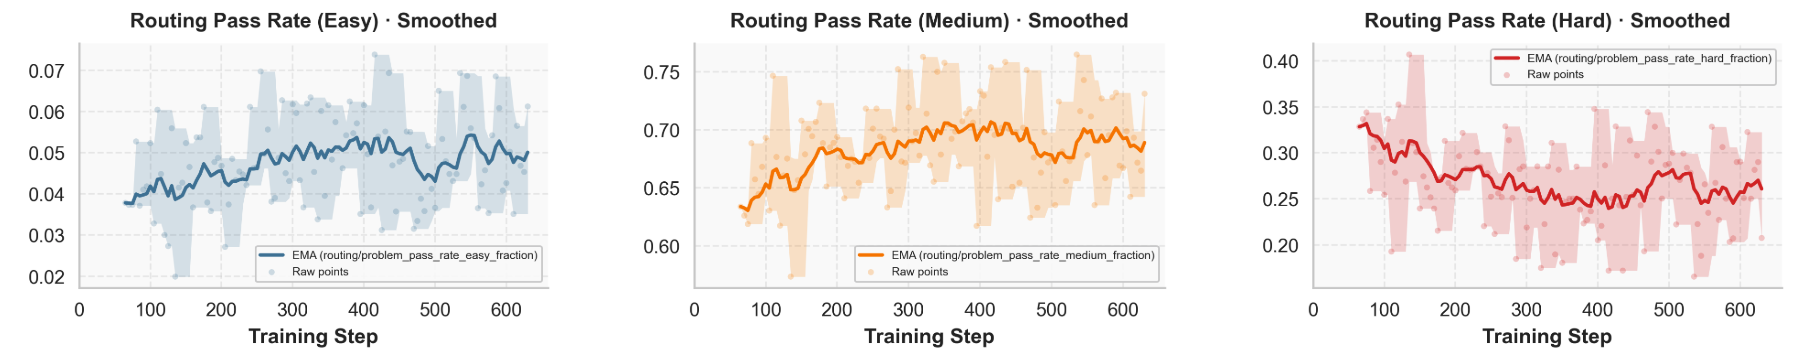
\includegraphics[width=1.1\textwidth]{Figures/drift_routing_dynamics.png}
    \caption{\textbf{Difficulty-routing dynamics (Qwen3-8B in tooluse)}}
    \label{fig:routing_dynamics}
\end{figure}

\subsection{Ablation Studies}

\paragraph{Component ablation.}
Figure~\ref{fig:tooluse_ablation} compares the mean@16 trajectories of DRIFT and two ablated variants on Tool Use. Although all variants improve rapidly at the beginning of training, their behavior diverges in the later stage. The complete method continues to improve and reaches the highest final accuracy, whereas removing difficulty routing leads to a sustained decline and removing the success buffer causes performance to plateau at a lower level. These results show that difficulty-aware signal allocation and historical success reuse are both important for stable long-term improvement.

\begin{figure}[tbp]
    \centering
    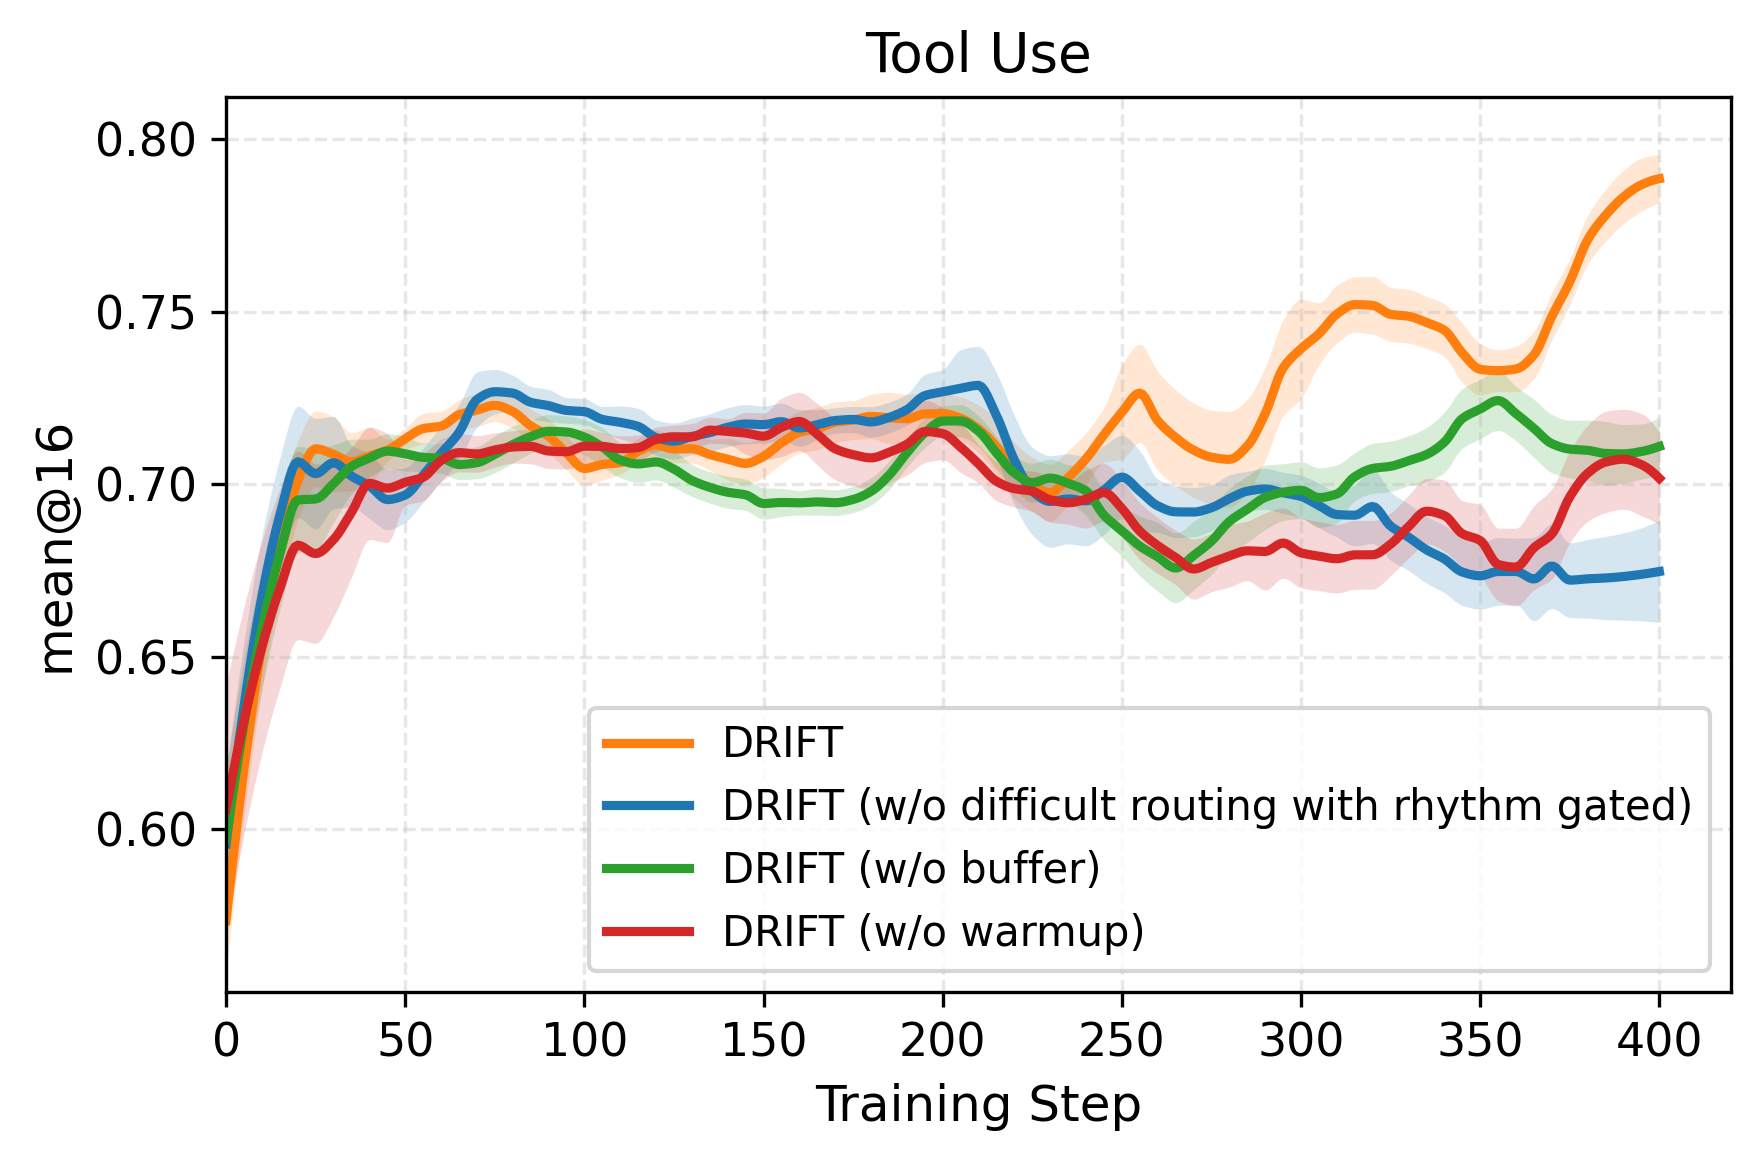
\includegraphics[width=0.78\textwidth]{Figures/drift_tooluse_ablation.png}
    \caption{\textbf{Ablation study on Tool Use of Qwen3-8B}}
    \label{fig:tooluse_ablation}
\end{figure}

\begin{table}[tbp]
\centering
\small
\caption{Ablation study of DRIFT on Qwen3-8B, reported as mean@16 accuracy (\%). \textbf{Bold} values indicate the best result, and \underline{underlined} values indicate the second-best result in each column.}
\label{tab:ablation_qwen3_8b}
\begin{tabular}{lcccccc}
\toprule
Method & Biology & Chemistry & Material & Physics & Tool Use & Average \\
\midrule
\textbf{Qwen3-8B} & 30.8 & 41.2 & 58.9 & 59.2 & 57.5 & 49.5 \\
+ SDPO & 64.8 & 78.9 & 76.1 & 72.7 & 67.7 & 72.0 \\
+ GRPO & 47.4 & 65.6 & 73.5 & 60.6 & 67.7 & 63.0 \\
\midrule
+ DRIFT w/o difficulty routing & \underline{66.2} & \underline{80.0} & 77.2 & 73.7 & \underline{73.4} & \underline{74.1} \\
+ DRIFT w/o success buffer & 64.9 & 79.9 & \underline{78.8} & \underline{77.8} & 73.2 & 74.9 \\
+ DRIFT w/o warm-up & 58.1 & 78.5 & 75.1 & 74.3 & 72.4 & 71.7 \\
\textbf{+ DRIFT (Ours)} & \textbf{74.4} & \textbf{82.0} & \textbf{81.4} & \textbf{80.5} & \textbf{79.2} & \textbf{79.5} \\
\bottomrule
\end{tabular}
\end{table}

\paragraph{Full ablation comparison.}
Table~\ref{tab:ablation_qwen3_8b} confirms that every major component of DRIFT contributes to the final performance. Removing difficulty routing reduces the average score from 79.5\% to 74.1\%, with especially clear drops on biology and tool use, indicating that problem-level allocation of RL and distillation signals is important for focusing optimization on the most learnable region. Removing the success buffer also causes a substantial degradation (74.9\% average), showing that cross-batch reuse of successful trajectories provides important privileged supervision when in-batch positives are sparse. The warm-up stage is likewise necessary: without it, performance falls to 71.7\%, and the drop is particularly severe on biology, suggesting that early-stage capability bootstrapping and buffer accumulation are critical for stable later optimization. Overall, the complete DRIFT design achieves the best result on all five benchmarks, showing that the gains come from the joint effect of curriculum warm-up, historical success reuse, and difficulty-aware routing rather than from any single component alone.

% ---- Section 6: Conclusion and Future Work ----
\section{Conclusion}
We identified a limitation shared by reinforcement learning and self-distillation approaches to LLM self-improvement: both lack a mechanism that tracks learning progress at the problem level and allocates optimization signals accordingly, so that easy problems keep receiving redundant updates, hard problems yield unreliable supervision, and high-value boundary cases remain under-explored. We then proposed DRIFT, an online self-evolution policy optimization framework that coordinates self-distillation and reinforcement learning according to the model's estimated mastery of each problem. At its core, Difficulty Routing uses smoothed historical pass rates to characterize problem-level learning state and to modulate the strength of reinforcement-learning updates, while Rhythm-Gated Structured Exploration refines credit assignment at the token level, concentrating exploratory updates on the critical reasoning positions that most directly determine correctness. We further introduced a Success Buffer that retains and reuses high-quality correct trajectories as privileged distillation references, and organized the whole process within a two-stage curriculum that progresses from rapid capability acquisition toward stable policy evolution.
Empirically, DRIFT consistently surpasses the peak performance of both GRPO and SDPO across all evaluated metrics, reaching an average accuracy of 79.5\% on five reasoning benchmarks and outperforming the strongest prior baseline by 2.1 points. The gains are most pronounced on tool use, where feedback is sparse and the decisive tokens are embedded in long trajectories—precisely the regime that DRIFT's privileged correction and rhythm-gated exploration are designed to address. DRIFT further generalizes across model families and scales: its advantage amplifies as the starting capability weakens, since the success buffer supplies privileged supervision exactly where reinforcement learning collapses for lack of positive samples, while its lead over the strongest baseline widens with model scale, consistent with self-teaching ability emerging as models grow.
More broadly, DRIFT suggests that effective self-evolution depends less on the choice between reinforcement learning and self-distillation than on when and where each signal is applied. By continually tracking what a model has already mastered and concentrating updates on the problems and the tokens that matter most, DRIFT turns a model's own successful experience into a stable, self-reinforcing source of supervision. We view problem-level learning-state tracking and token-level credit shaping as general principles for self-evolution, and hope they inform future methods that let language models improve from their own experience without external expert supervision.


% ---- Section 7: References ----
\bibliographystyle{iclr2026_conference}
\bibliography{references}

% ---- Section 8: Appendix (Later) ----
\appendix
\section{Appendix}

\begin{figure}[H]
    \centering
    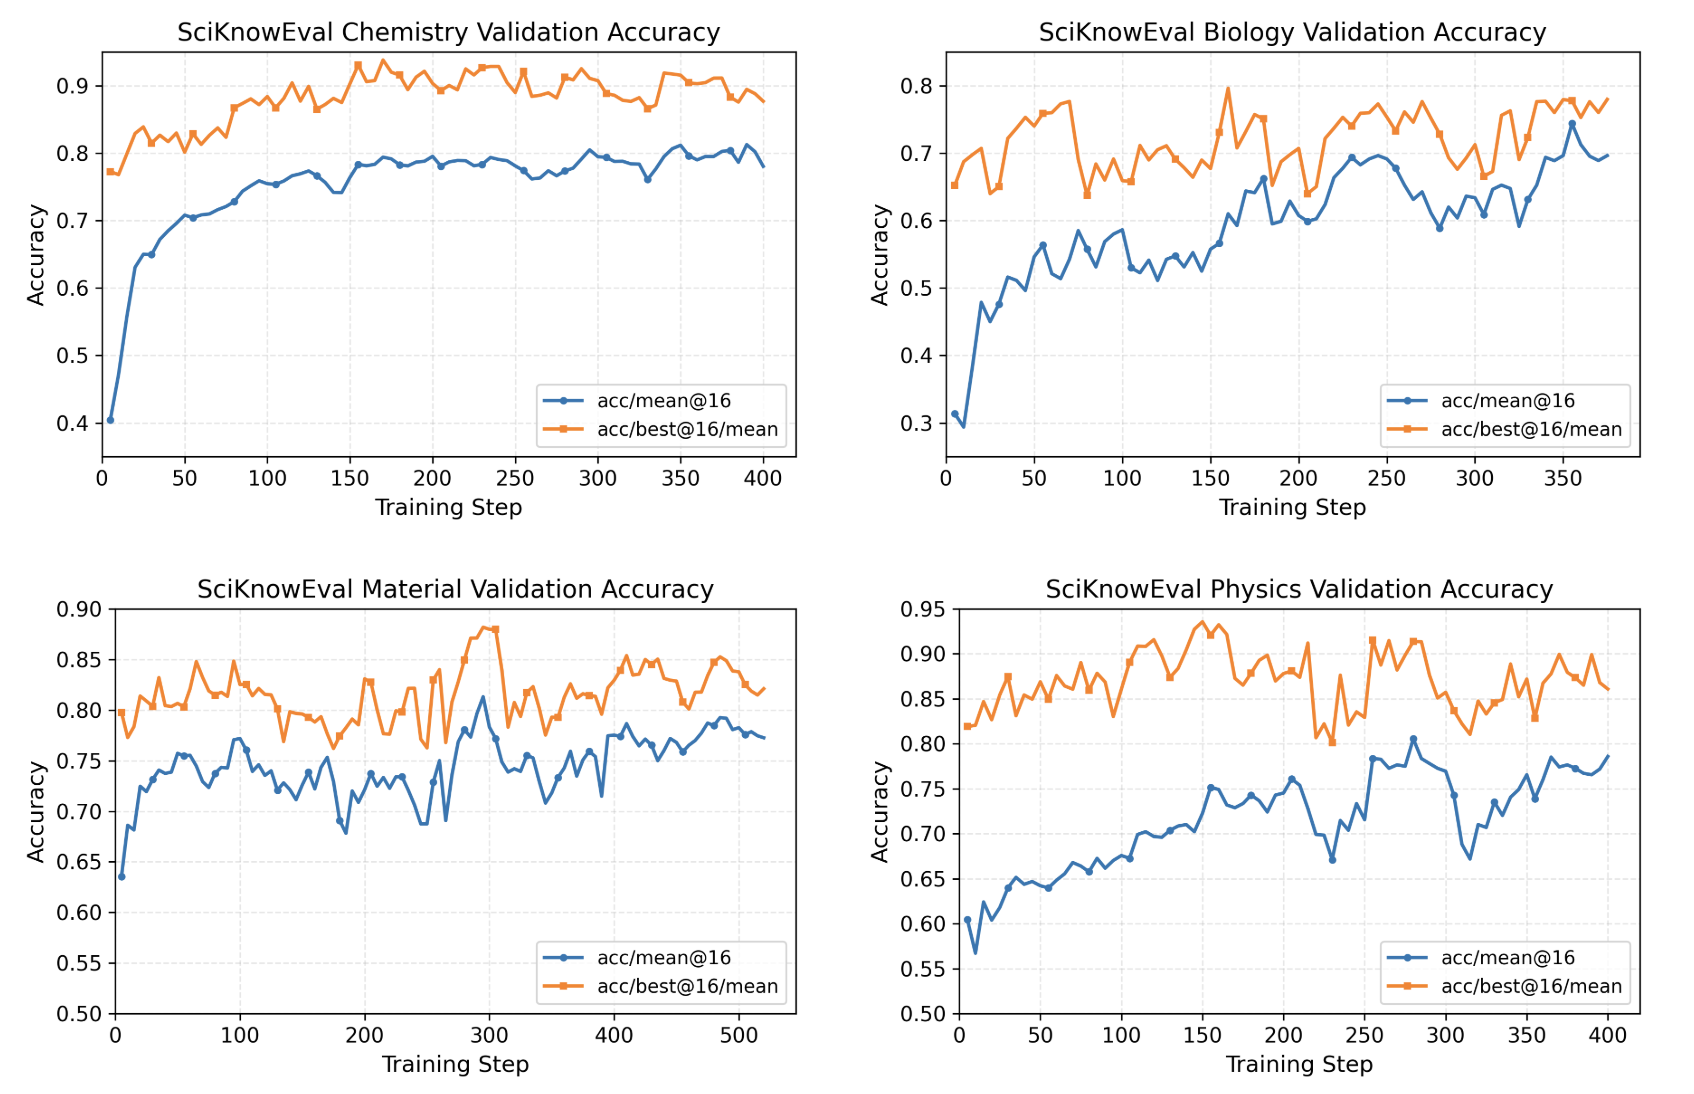
\includegraphics[width=0.90\textwidth]{Figures/drift_sciknoweval_validation.png}
    \caption{\textbf{Validation performance on the STEM datasets.} In addition to improvements in mean@16, best@16 also increases steadily throughout training.}
    \label{fig:appendix_sciknoweval_validation}
\end{figure}

\begin{table}[H]
    \centering
    \small
    \caption{\textbf{Best@16 performance on Qwen3-8B.} DRIFT outperforms SDPO and GRPO across all five tasks, with particularly pronounced gains on materials and tool use.}
    \label{tab:appendix_best16_comparison}
    \begin{tabular}{lccccc}
        \toprule
        Method & Biology & Chemistry & Material & Physics & Tool Use \\
        \midrule
        SDPO  & 78.8 & 89.4 & 80.4 & 91.6 & 73.4 \\
        GRPO  & 80.0 & 93.5 & 82.9 & 87.2 & 70.8 \\
        \textbf{DRIFT} & \textbf{80.1} & \textbf{94.3} & \textbf{87.9} & \textbf{93.8} & \textbf{83.7} \\
        \bottomrule
    \end{tabular}
\end{table}

\end{document}
